\chapter{Analysis of the Impacts of Heterogeneity Losses due to Upscaling in Well Testing Simulations}
\label{chapter-AIHLUWTS}

Chapters \ref{chapter-mathematical-formulation} to \ref{chapter-solution} show how the reservoir simulator utilized in this project has been developed and validated.
%
Chapters \ref{chapter-upscaling} and \ref{chapter-well-testing} show introductions of upscaling and well testing, the areas investigated by this project.
%
This chapter shows the analysis of the effects of upscaling in well testing simulations, the main application of the simulator developed in this project.
%
Several models have been created and put under flow simulation.
%
The results of bottom hole pressure, pressure drop, and Bourdet derivative have been plotted and compared.
%
The idea is to visualize how a numerical model for a pressure transient analysis would provide different results for a fine grid versus an upscaled one.
%
This chapter's first section shows details of each of those models and the parameters of the simulation.
%
The last section will show the results obtained in the simulation and its analyzes.

\section{Models}

Eight different cases have been created and simulated for outputting bottom hole pressure, pressure drop, and the Bourdet derivative.
%
They are parallelepipedal models of artificial sandstone reservoirs.
%
Table \ref{table-common-characteristics-for-simulation-cases} shows the common characteristics for all the cases.
%
The fluid model for all the scenarios is the same as utilized in the validation cases, illustrated by Figure \ref{figure-fluid-proprieties}.
%
The porosity-permeability relationship is equal for all the models and follows the correlation illustrated in Figure \ref{figure-porosity-permeability-relationship} and in the Eq. \ref{equation-porosity-permeability-relationship}.
%
\begin{table}[htbp]
	\centering
	\caption{Common characteristics for all the simulation cases.}
	\begin{tabular}{c c}
		\toprule
		Parameter & Value (if applicable)\\
		\midrule
		Reservoir length in the $x$ direction & 2559.03 ft\\
		Reservoir length in the $y$ direction & 2559.03 ft\\
		Reservoir length in the $z$ direction & 164.04 ft\\
		Boundary conditions & Sealed reservoir \\
		Well & Vertical well in the\\
		& center of the reservoir\\
		Completions & From the top to the\\
		& bottom of the reservoir\\
		Average porosity & 20\%\\
		Average horizontal permeability & 51.59 mD\\
		Average vertical permeability & 51.59 mD\\
		Formation compressibility & $1.31 x 10^{-4}$ psi$^{-1}$\\
		Fluid compressibility &  1.41 x 10$^{-5}$ psi$^{-1}$\\
		Depth of the topmost layer & 10,498.69 ft\\
		Reference depth for the initial pressure & 10,498.69 ft\\
		Initial pressure at the reference depth & 3,916.01 psi\\
		Well radius & 6 in\\
		Skin factor & -0.5\\
		\bottomrule
	\end{tabular}
	\label{table-common-characteristics-for-simulation-cases}
\end{table}
%
\begin{figure}[H]
	\centering
	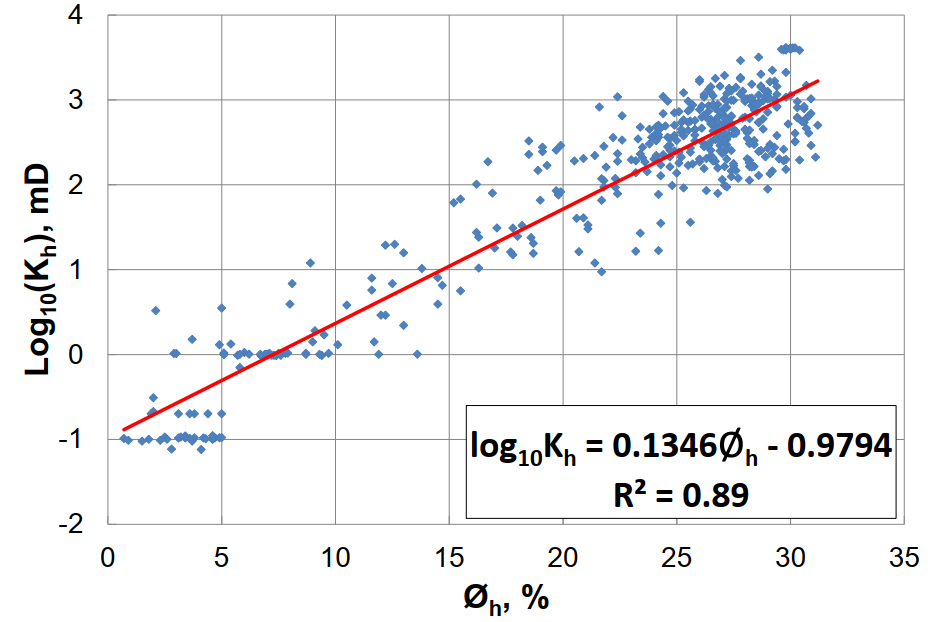
\includegraphics[width=0.8\linewidth]{figure-porosity-permeability-relationship.png}
	\caption{Relationship between the porosity and permeability of the UNISIM-I, a synthetic sandstone model based on the Namorado Field, Campos Basin of Brazil. Source: \cite{Avansi2015}. The eight models constructed in this chapter have the same porosity-permeability relationship, as shown in this picture.}
	\label{figure-porosity-permeability-relationship}
\end{figure}
%
\begin{equation}\label{equation-porosity-permeability-relationship}
	k_h = 10^{(0.1346\phi)-0.9794}.
\end{equation}
%
In other words, Table \ref{table-common-characteristics-for-simulation-cases}, Figure \ref{figure-fluid-proprieties}, Figure \ref{figure-porosity-permeability-relationship} and Eq. \ref{equation-porosity-permeability-relationship} shows the common characteristics shared between the eight models.
%
What differs one case to another is the size and number of the grid blocks and the standard deviation of the porosity and permeability. 

Scenarios 1 and 2 are homogeneous in terms of porosity and permeability.
%
While scenario 1 has a fine grid, scenario two has a coarse grid constructed by the upscaling of scenario 1.
%
In other words, scenario 2 is the upscaled version of scenario 1.
%
Each direction of scenario 2 presents half the number of grid blocks in comparison to scenario 1.
%
Since scenario 1 is homogeneous, there is no spatial variation of porosity and permeability and scaling up can be done straightforwardly, without the need for averaging techniques.

Scenario 3 has heterogeneous permeabilities and porosities.
%
The porosity is populated by utilizing a normal distribution with a mean equals to 20\%, the same as scenario 1, and a standard deviation equals 3\%.
%
Then, the horizontal permeabilities are calculated by utilizing the correlation shown in Eq. \ref{equation-porosity-permeability-relationship}.
%
Finally, the vertical permeabilities are set to be equals to 10\% of the horizontal for each grid bock.
%
Thus, both the horizontal and vertical permeabilities follow log-normal distributions with the same means as in scenario 1.
%
Scenario 4 is the upscaled version of scenario 3.
%
Since porosity and permeability are not homogeneous, it is necessary to perform an upscaling technique.
%
A simple volumetric averaging has been utilized for upscaling the porosity, as shown in Eq. \ref{equation-upscaling-porosity}.
%
An arithmetic-harmonic averaging has been utilized for scaling up the permeability tensor, as demonstrated by Eq. \ref{equation-arithmetic-harmonic-averaging}.

Scenario 5 is essentially the same as scenario 3, with the difference that the standard deviation of the porosity is set to be equal to 6\%, the double of the one from scenario 3.
%
That would result in permeabilities with higher standard deviations as well since they are populated by following the same rules as in scenario 3.
%
Scenario 6 is scenario 5 upscaled by the same approach described above.

Scenario 7 is scenario 3, with a standard deviation of porosity that equals 1.5\%, half of the one from scenario 3.
%
Again, the permeabilities have been populated in the same way as described above.
%
Finally, the last scenario, 8, is the upscaled version of scenario 7.
%
Table \ref{table-differences-between-simulation-cases} summarizes the differences between each model:
%
\begin{table}[htbp]
	\centering
	\caption{Difference between each simulation scenario.}
	\label{table-differences-between-simulation-cases}
	\begin{tabular}{c c c c c c c}
		\toprule
		Case & Nx & Ny & Nz & Upscaling & Heterogeneity & $\phi$ Standard Deviation\\
		\midrule
		1 & 26 & 26 & 20 & No & Homogeneous & 0\\
		2 & 13 & 13 & 10 & No & Homogeneous & 0\\
		3 & 26 & 26 & 20 & Yes & Heterogeneous & 3\%\\
		4 & 13 & 13 & 10 & Yes & Heterogeneous & 6\%\\
		5 & 26 & 26 & 20 & Yes & Heterogeneous & 6\%\\
		6 & 13 & 13 & 10 & Yes & Heterogeneous & 6\%\\
		7 & 26 & 26 & 20 & Yes & Heterogeneous & 1.5\%\\
		8 & 13 & 13 & 10 & Yes & Heterogeneous & 1.5\%\\
		\bottomrule
	\end{tabular}
\end{table}

Appendix \ref{appendix-models-descriptions} shows in more detail the porosity-permeability distributions of scenarios 3 to 8.
%
The next section shows the results obtained by the simulation done in those models.

\section{Results}

The previous section displays the details of the eight models constructed for this study.
%
All those cases have been put under flow simulation for a drawdown test scenario.
%
The well is initially closed and opens at the time of 0.1 days with a constant flow rate.
%
Then, the simulation continues until time is equal to 2 days.
%
Figure \ref{figure-AIHLUWTS-flow-rates} shows the flow rate variation in this test:
%
\begin{figure}[H]
	\centering
	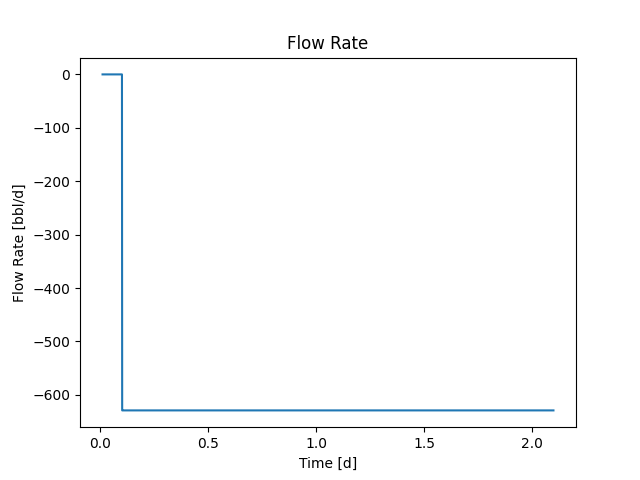
\includegraphics[width=0.9\linewidth]{figure-AIHLUWTS-flow-rates.png}
	\caption{Well flow rate for all the cases in the simulation. Negative values indicate production.}
	\label{figure-AIHLUWTS-flow-rates}
\end{figure}
\noindent
%
This increase in flow rate implies a variation in the bottom hole pressure.
%
Figure \ref{figure-bottom-hole-pressure-fine-models} shows the BHP for all the fine models.
%
\begin{figure}[H]
	\centering
	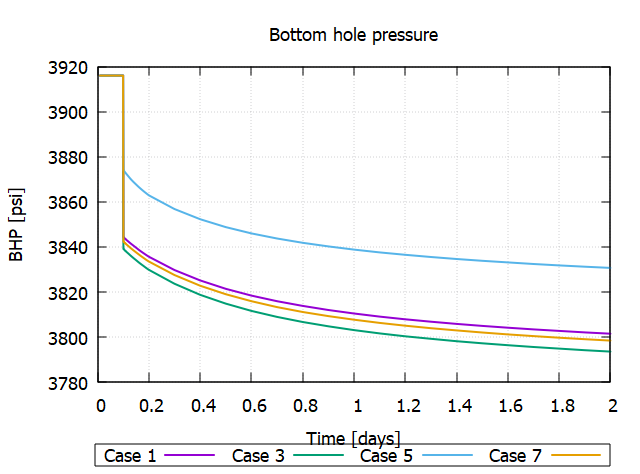
\includegraphics[width=0.9\linewidth]{figure-bottom-hole-pressure-fine-models.png}
	\caption{Bottom hole pressure for the fine models (case 1, case 3, case 5, and case 7).}
	\label{figure-bottom-hole-pressure-fine-models}
\end{figure}
\noindent
%
One could see that the results for the homogeneous model (case 1) were very similar to the ones of the model with a lower standard deviation (case 7).
%
The BHP for case 5 (higher standard deviation) was considerably higher than those for the cases with lower dispersions.
%
Thus, the porosity-permeability dispersion can change the bottom-hole pressure results in a well test. 

Figures \ref{figure-bottom-hole-pressure-cases-1-2} to \ref{figure-bottom-hole-pressure-cases-7-8} display the outputs of BHP for the simulations, for each pair of fine-grid model and its upscaled version.
%
\begin{figure}[H]
	\centering
	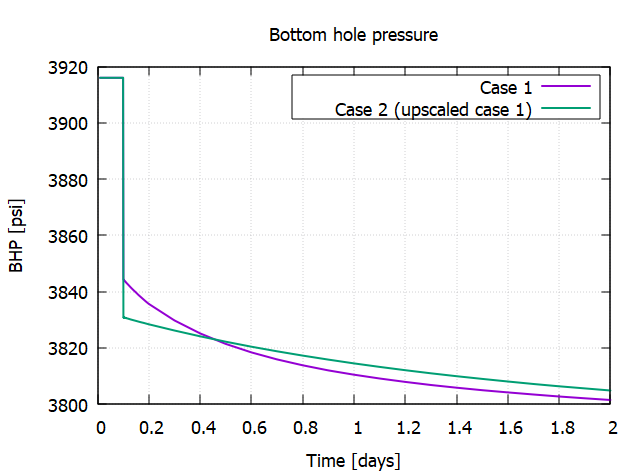
\includegraphics[width=0.9\linewidth]{figure-bottom-hole-pressure-cases-1-2.png}
	\caption{Bottom hole pressure for case 1 and its upscaled version, case 2.}
	\label{figure-bottom-hole-pressure-cases-1-2}
\end{figure}
\noindent
%
Figure \ref{figure-bottom-hole-pressure-cases-1-2} above shows the BHP for case 1 and case 2 (the upscaled version of case 1).
%
One could see that the results are quite similar from one case to another, as both cases present homogeneous porosity and permeability.
%
In the drawdown period, the bottom-hole pressure for case 2 fits inside the range of maximum-minimum BHP for case 1.
%
One possible explanation for this result is that, since case 1 has a larger number of grid-blocks than case 2, the pressure transient propagates more continuously the grid in case 1 than in case 2.
%
\begin{figure}[H]
	\centering
	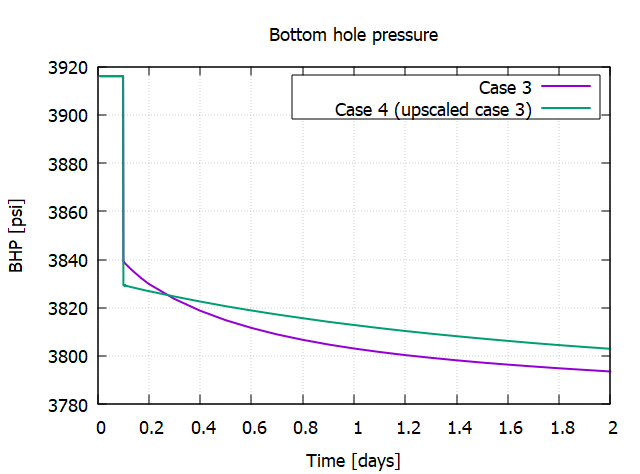
\includegraphics[width=0.9\linewidth]{figure-bottom-hole-pressure-cases-3-4.png}
	\caption{Bottom hole pressure for case 3 and its upscaled version, case 4.}
	\label{figure-bottom-hole-pressure-cases-3-4}
\end{figure}
\noindent
%
Figure \ref{figure-bottom-hole-pressure-cases-3-4} shows the results for case 3 and its upscaled version, case 4.
%
Differently than cases 1 and 2, cases 3 and 4 are heterogeneous reservoirs.
%
Thus, the arithmetic-harmonic technique has been utilized in the upscaling for generating case 4.
%
The difference between the curves is higher in cases 3 and 4 than in cases 1 and 2.
%
Nevertheless, this difference is still small, showing that the arithmetic-averaging upscaling represented the fine model with reasonably good accuracy.
%
\begin{figure}[H]
	\centering
	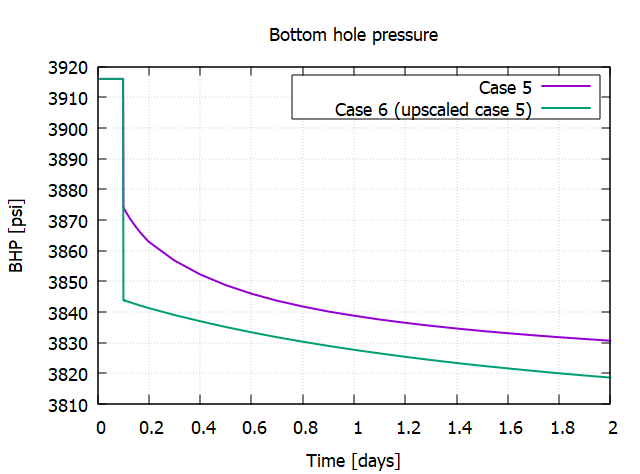
\includegraphics[width=0.9\linewidth]{figure-bottom-hole-pressure-cases-5-6.png}
	\caption{Bottom hole pressure for case 5 and its upscaled version, case 6.}
	\label{figure-bottom-hole-pressure-cases-5-6}
\end{figure}
\noindent
%
Figure \ref{figure-bottom-hole-pressure-cases-5-6} above shows the results for case 5 and its upscaled version, case 6.
%
Those are the cases with the higher standard deviation of porosity and, consequently, permeability.
%
As shown by the image above, those are also the cases with the highest difference between the curves for the fine-grid and upscaled models.
%
\begin{figure}[H]
	\centering
	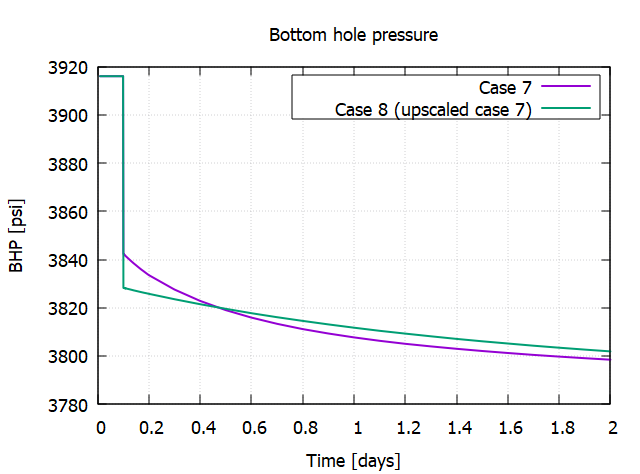
\includegraphics[width=0.9\linewidth]{figure-bottom-hole-pressure-cases-7-8.png}
	\caption{Bottom hole pressure for case 7 and its upscaled version, case 8.}
	\label{figure-bottom-hole-pressure-cases-7-8}
\end{figure}
\noindent
%
Figure \ref{figure-bottom-hole-pressure-cases-7-8} displays the same information for cases 7 and 8.
%
Those are the heterogeneous models with the lowest standard deviation in porosity and permeability.
%
Those are also the cases in which the curves are closer to the upscaled model and its fine-grid counterpart.
%
Looking at the previous four images, Figures \ref{figure-bottom-hole-pressure-cases-1-2} to Figure \ref{figure-bottom-hole-pressure-cases-7-8}, one could see that the difference between bottom-hole pressure for the fine-grid and coarse-grid models is consistently greater when the standard deviations in the porosity-permeability are higher.

Next, Figure \ref{figure-log-log-plot-fine-models} below shows the diagnostic log-log plot of the pressure drop and the Bourdet derivative against the elapsed time for the fine-grid models, cases 1, 3, 5, and 7.
%
\begin{figure}[H]
	\centering
	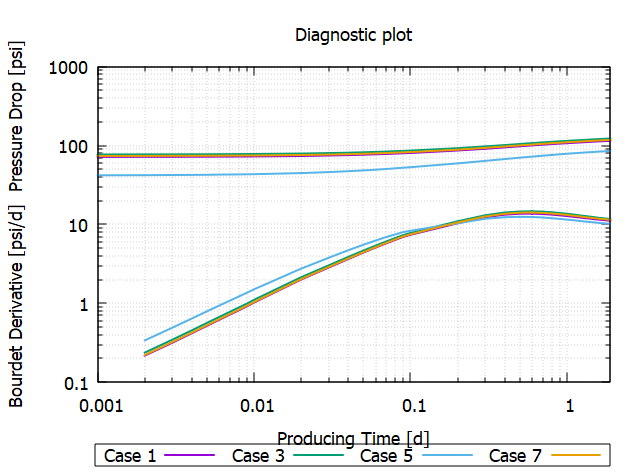
\includegraphics[width=0.8\linewidth]{figure-log-log-plot-fine-models.png}
	\caption{Pressure drop and Bourdet derivative for the fine-grid models (case 1, case 3, case 5, and case 7).}
	\label{figure-log-log-plot-fine-models}
\end{figure}
\noindent
%
Looking at the figure above, one could see that the curves of cases 1, 3, and 7 are very close one to another.
%
Case 5 presents lower pressure drops and higher Bourdet derivatives than the other scenarios due to its higher standard deviation.
%
The next four figures,\ref{figure-log-log-plot-cases-1-2} to \ref{figure-log-log-plot-cases-7-8}, show this diagnostic plot for each pair of fine-grid/upscaled models.
%
\begin{figure}[H]
	\centering
	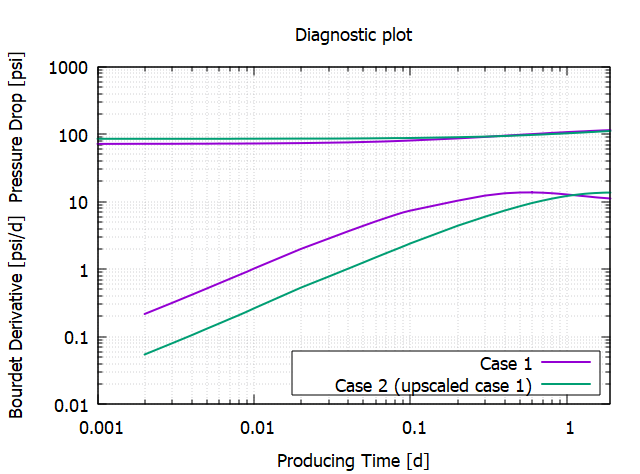
\includegraphics[width=0.8\linewidth]{figure-log-log-plot-cases-1-2.png}
	\caption{Pressure drop and Bourdet derivative for case 1 and its upscaled version, case 2.}
	\label{figure-log-log-plot-cases-1-2}
\end{figure}
%
\begin{figure}[H]
	\centering
	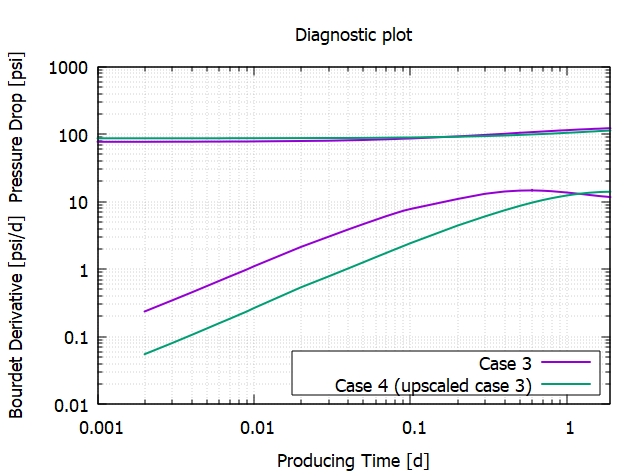
\includegraphics[width=0.8\linewidth]{figure-log-log-plot-cases-3-4.png}
	\caption{Pressure drop and Bourdet derivative the case 3 and its upscaled version, case 4.}
	\label{figure-log-log-plot-cases-3-4}
\end{figure}
%
\begin{figure}[H]
	\centering
	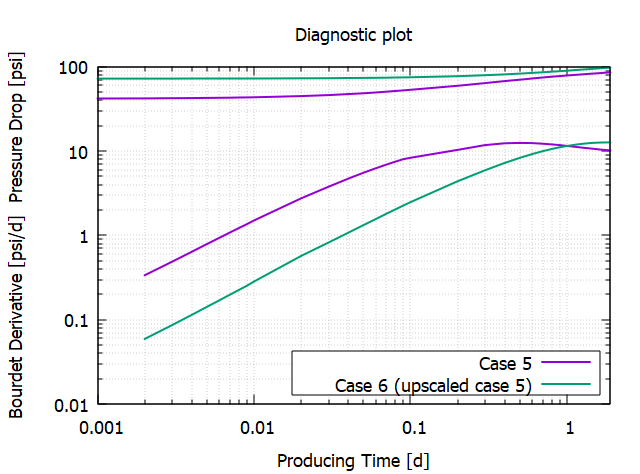
\includegraphics[width=0.8\linewidth]{figure-log-log-plot-cases-5-6.png}
	\caption{Pressure drop and Bourdet derivative the case 5 and its upscaled version, case 6.}
	\label{figure-log-log-plot-cases-5-6}
\end{figure}
%
\begin{figure}[H]
	\centering
	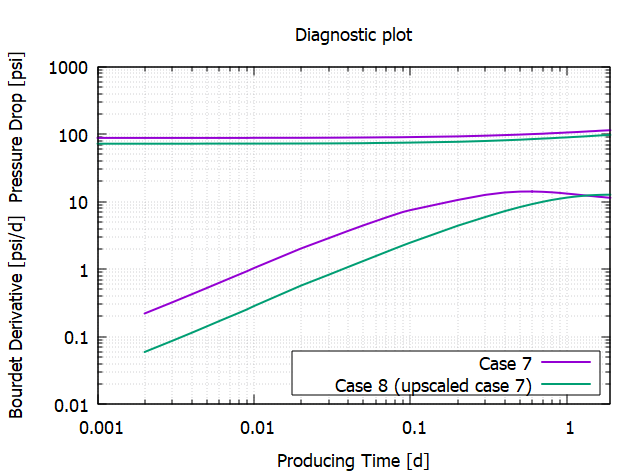
\includegraphics[width=0.8\linewidth]{figure-log-log-plot-cases-7-8.png}
	\caption{Pressure drop and Bourdet derivative the case 7 and its upscaled version, case 8.}
	\label{figure-log-log-plot-cases-7-8}
\end{figure}
\noindent
%
The images above show pressure drop curves very close to each other.
%
However, they also show a considerable difference between the Bourdet derivative curves for the fine-grid models and their upscaled version.
%
In the rightmost part of the Bourdet derivative curves, it seems like the fine-grid models show a slightly negative decline while their upscale versions do not.
%
This discrepancy is higher for cases with higher standard deviations.
%
Since there are techniques of pressure transient analysis that evaluate the slope in this area of the Bourdet derivative curve (for example, describing the flow regime), the discrepancy between simulations of fine-grid models and their upscaled versions could lead to misinterpretations in well testing.
%
Nevertheless, more profound studies are made necessary for analyzing this possibility.
